
\documentclass[ review  , 3p ]{elsarticle}
%default = preprint (single sapce), review = doublespace
%detail class option: https://www.elsevier.com/__data/assets/pdf_file/0008/56843/elsdoc-1.pdf

% eliminate "Preprinted to Elsevier"
\makeatletter
\def\ps@pprintTitle{%
 \let\@oddhead\@empty
 \let\@evenhead\@empty
 \def\@oddfoot{\centerline{\thepage}}%
 \let\@evenfoot\@oddfoot}
\makeatother

%%% Begin My package additions %%%%%%%%%%%%%%%%%%%
\usepackage[hyphens]{url}



\usepackage{lineno} % add
\providecommand{\tightlist}{%
  \setlength{\itemsep}{0pt}\setlength{\parskip}{0pt}}

\usepackage{graphicx}
\usepackage{booktabs} % book-quality tables

\usepackage{zxjatype}
\setCJKmainfont[BoldFont = IPAゴシック]{IPA明朝}
\setCJKsansfont{IPAゴシック}
\setCJKmonofont{IPAゴシック}

\usepackage{threeparttable}
\usepackage{color}

%\usepackage{xpatch}
%\xpatchcmd{\MaketitleBox}{\hrule}{}{}{}% remove first horizontal rule (above abstract)
%\xpatchcmd{\MaketitleBox}{\hrule}{}{}{}% remoce second horizonral rule (below keywords)
%%%%%%%%%%%%%%%% end my additions to header

\usepackage[T1]{fontenc}
\usepackage{lmodern}
\usepackage{amssymb,amsmath}
\usepackage{ifxetex,ifluatex}
\usepackage{fixltx2e} % provides \textsubscript
% use upquote if available, for straight quotes in verbatim environments
\IfFileExists{upquote.sty}{\usepackage{upquote}}{}
\ifnum 0\ifxetex 1\fi\ifluatex 1\fi=0 % if pdftex
  \usepackage[utf8]{inputenc}
\else % if luatex or xelatex
  \usepackage{fontspec}
  \ifxetex
    \usepackage{xltxtra,xunicode}
  \fi
  \defaultfontfeatures{Mapping=tex-text,Scale=MatchLowercase}
  \newcommand{\euro}{€}
\fi
% use microtype if available
\IfFileExists{microtype.sty}{\usepackage{microtype}}{}
\bibliographystyle{elsarticle-harvard}
\usepackage{longtable}
\usepackage{tabularx}
\ifxetex
  \usepackage[setpagesize=false, % page size defined by xetex
              unicode=false, % unicode breaks when used with xetex
              xetex]{hyperref}
\else
  \usepackage[unicode=true]{hyperref}
\fi
\hypersetup{breaklinks=true,
            bookmarks=true,
            pdfauthor={},
            pdftitle={Short Paper},
            colorlinks=false,
            urlcolor=blue,
            linkcolor=magenta,
            pdfborder={0 0 0}}
\urlstyle{same}  % don't use monospace font for urls

\setcounter{secnumdepth}{5}

\newlength{\cslhangindent}
\setlength{\cslhangindent}{1.5em}
\newlength{\csllabelwidth}
\setlength{\csllabelwidth}{3em}
\newenvironment{CSLReferences}[3] % #1 hanging-ident, #2 entry spacing
 {% don't indent paragraphs
  \setlength{\parindent}{0pt}
  % turn on hanging indent if param 1 is 1
  \ifodd #1 \everypar{\setlength{\hangindent}{\cslhangindent}}\ignorespaces\fi
  % set entry spacing
  \ifnum #2 > 0
  \setlength{\parskip}{#2\baselineskip}
  \fi
 }%
 {}
\usepackage{calc} % for \widthof, \maxof
\newcommand{\CSLBlock}[1]{#1\hfill\break}
\newcommand{\CSLLeftMargin}[1]{\parbox[t]{\maxof{\widthof{#1}}{\csllabelwidth}}{#1}}
\newcommand{\CSLRightInline}[1]{\parbox[t]{\linewidth}{#1}}
\newcommand{\CSLIndent}[1]{\hspace{\cslhangindent}#1}

% Pandoc toggle for numbering sections (defaults to be off)


% Pandoc header


\begin{document}
  \begin{frontmatter}

    \title{Charitable Giving, Tax Reform, and Government Efficiency\tnoteref{1}}
            \tnotetext[1]{This research is base on}
                \author[Osaka University]{
      Hiroki Kato 
       \corref{*} }
     \ead{vge008kh@stundent.econ.osaka-u.ac.jp}   %to avoid auto-link, use \@ instead of @
        \author[Chiba University]{
      Tsuyoshi Goto 
      }
      %to avoid auto-link, use \@ instead of @
        \author[Kobe University]{
      Yong-Rok Kim 
      }
      %to avoid auto-link, use \@ instead of @
            \address[Osaka University]{Graduate School of Economics, Osaka University, Japan}
        \address[Chiba University]{Graduate School of Economics, Chiba University, Japan}
        \address[Kobe University]{Graduate School of Economics, Kobe University, Japan}
            \cortext[*]{Corresponding Author.}
      
        \begin{abstract}
      Brah
    \end{abstract}
      
        \begin{keyword}
      Charitable giving, Giving price, Tax reform, Governement efficiency, South Korea
       \JEL{D91, I10, I18} 
    \end{keyword}
    
  \end{frontmatter}

  \hypertarget{introduction}{%
  \section{Introduction}\label{introduction}}

  \hypertarget{background-of-south-korea-tax-reform}{%
  \subsection{Background of South Korea Tax Reform}\label{background-of-south-korea-tax-reform}}

  To investigate the price effect, we use the 2014 tax reform in the South Korea
  (Bursztyn and Jensen, 2017).

  \begin{itemize}
  \tightlist
  \item
    Before 2014, tax deduction was adopted to subsidize charitable donation behavior.
  \item
    After 2014, tax credit have been adopted.
  \end{itemize}

  The main difference is that tax credits reduce taxes directly, while tax deductions indirectly lower the tax burden by decreasing the taxpayer's marginal tax rate, which increases with gross income

  \hypertarget{data}{%
  \section{Data}\label{data}}

  \hypertarget{national-survey-of-tax-and-benefit-nastab}{%
  \subsection{National Survey of Tax and Benefit (NaSTaB)}\label{national-survey-of-tax-and-benefit-nastab}}

  \begin{itemize}
  \tightlist
  \item
    The Korea Institute of Taxation and Finance implements the financial panel survey to study the tax burden of households and the benefits that households receive from goverment.
  \item
    The subjects of this survey are general household and household members living in 15 cities and provinces nationwide.
  \item
    This survey is based on a face-to-face interview. If it is difficult for investigators to meet subjects, another family member answers on behalf of him.
  \item
    Survey items: Annual taxable income (last year), charitable donations (last year), trust for politicians (5-Likert scale), and other covariates (age, education, gender etc.).
  \item
    Survey period: 2008 \textasciitilde{} 2019

    \begin{itemize}
    \tightlist
    \item
      We use survey data after 2013 to focus on tax policy change in 2014.
    \end{itemize}
  \end{itemize}

  \hypertarget{time-series-of-chariable-giving}{%
  \subsection{Time Series of Chariable Giving}\label{time-series-of-chariable-giving}}

  \begin{figure}

  {\centering 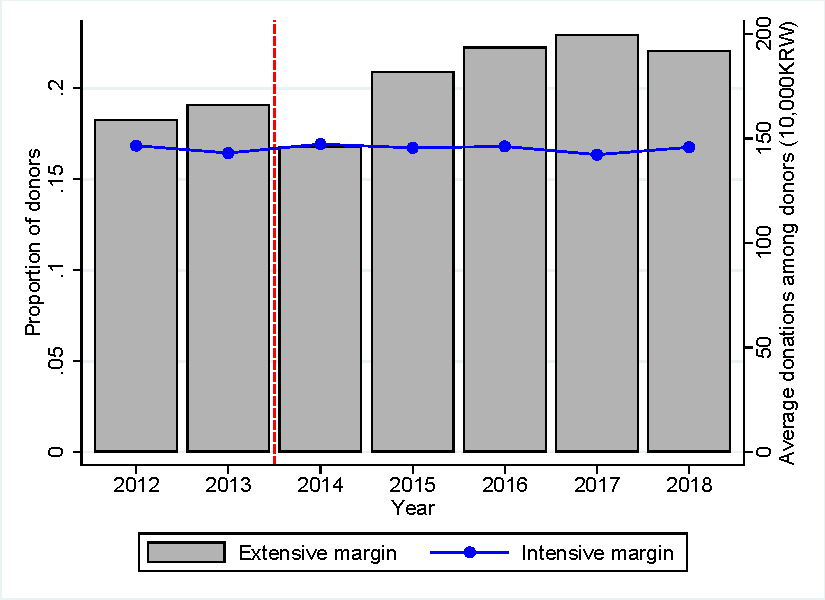
\includegraphics[width=0.9\linewidth]{C:/Users/katoo/Desktop/NASTAB/_assets/SummaryOutcome} 

  }

  \caption{Proportion of Donors and Average Donations among Donors}\label{fig:unnamed-chunk-1}
  \end{figure}

  \hypertarget{summary-statistics-of-covariates}{%
  \subsection{Summary Statistics of Covariates}\label{summary-statistics-of-covariates}}

  \begin{table}

  \caption{\label{tab:kableSummaryCovariate}Summary Statistics of Covariates}
  \centering
  \begin{tabular}[t]{lcccc}
  \toprule
   & 2012 & 2013 & 2014 & 2015\\
  \midrule
  Female & 0.51 & 0.51 & 0.52 & 0.52\\
  Age & 38.39 & 39.10 & 39.67 & 40.51\\
  Annual taxable income & 1699.86 & 1764.04 & 1838.76 & 1872.54\\
  University graduate & 0.28 & 0.28 & 0.29 & 0.30\\
  High school graduate & 0.30 & 0.30 & 0.31 & 0.31\\
  \#.Respondents & 14138 & 13984 & 13787 & 13524\\
  \#.Households & 4756 & 4807 & 4819 & 4832\\
  \bottomrule
  \end{tabular}
  \end{table}

  \hypertarget{summary-statistics-of-covariates-contd}{%
  \subsection{Summary Statistics of Covariates (Cont'd)}\label{summary-statistics-of-covariates-contd}}

  \begin{table}

  \caption{\label{tab:kableSummaryCovariate2}Summary Statistics of Covariates (Continued)}
  \centering
  \begin{tabular}[t]{lccc}
  \toprule
   & 2016 & 2017 & 2018\\
  \midrule
  Female & 0.52 & 0.52 & 0.52\\
  Age & 41.07 & 41.89 & 42.55\\
  Annual taxable income & 1906.91 & 1951.55 & 2039.47\\
  University graduate & 0.31 & 0.33 & 0.34\\
  High school graduate & 0.31 & 0.31 & 0.31\\
  \#.Respondents & 13238 & 12963 & 12795\\
  \#.Households & 4790 & 4770 & 4765\\
  \bottomrule
  \end{tabular}
  \end{table}

  \hypertarget{what-is-giving-price}{%
  \subsection{What is Giving Price?}\label{what-is-giving-price}}

  Consider allocation between private consumptions (\(x_i\)) and charitable giving (\(g_i\)).
  Let \(y_i\) be pre-tax total income.
  Then, the budget constraint is

  \[
      x_i + g_i = y_i - T_i(y_i, g_i),
  \]

  where \(T_i\) is tax amount depending on the pre-tax income and charitable giving.

  \hypertarget{determination-of-tax-amount}{%
  \subsection{Determination of Tax Amount}\label{determination-of-tax-amount}}

  Tax deduction reduces taxable income by giving, that is,

  \[
      T_i = \tau(y_i - g_i) \cdot (y_i - g_i),
  \]

  where \(\tau(\cdot)\) is the marginal income tax rate which is determined by \(y_i - g_i\).

  Tax credit reduces tax amount directly, that is,

  \[
      T_i = \tau(y_i)\cdot y_i - m g_i,
  \]

  where \(m \in [0, 1]\) is the tax credit rate.

  \hypertarget{derive-giving-price}{%
  \subsection{Derive Giving Price}\label{derive-giving-price}}

  Under the tax deduction system, the budget constraint is

  \[
      x_i + [1 - \tau(y_i - g_i)]g_i = [1 - \tau(y_i - g_i)] y_i.
  \]

  Thus, the giving price of tax deduction system is \(p_i^{d} = 1 - \tau(y_i - g_i)\).

  Under the tax credit system, the budget constraint is

  \[
      x_i + (1 - m) g_i = [1 - \tau(y_i)] y_i.
  \]

  Thus, the giving price of tax credit system is \(p_i^c = 1 - m\).

  \hypertarget{construct-giving-price}{%
  \subsection{Construct Giving Price}\label{construct-giving-price}}

  In the South Korea, the tax policy about charitable giving drastically changed in 2014.

  \begin{itemize}
  \tightlist
  \item
    tax deduction (before 2014): \(\text{Price}_i = 1 - \tau(y_i - g_i)\)

    \begin{itemize}
    \tightlist
    \item
      the giving price is endogenous because people can manipulate \(\tau(y_i - g_i)\) using the charitable giving \(g_i\). Since this problem is caused by \emph{last} donations, we use the giving price applying to the \emph{first} donations (\textbf{first price}). The first price is calculate by \(\tau(y_i)\) where \(y_i\) is the annual taxable income reported in the NaSTaB.
    \end{itemize}
  \item
    tax credit (after 2014): \(\text{Price}_i = 1 - m\)

    \begin{itemize}
    \tightlist
    \item
      In the South Korea, the tax credit rate determines exogeneity, \(m = 0.15\).
    \end{itemize}
  \end{itemize}

  \hypertarget{income-distribution-and-giving-price}{%
  \subsection{Income Distribution and Giving Price}\label{income-distribution-and-giving-price}}

  \begin{figure}

  {\centering 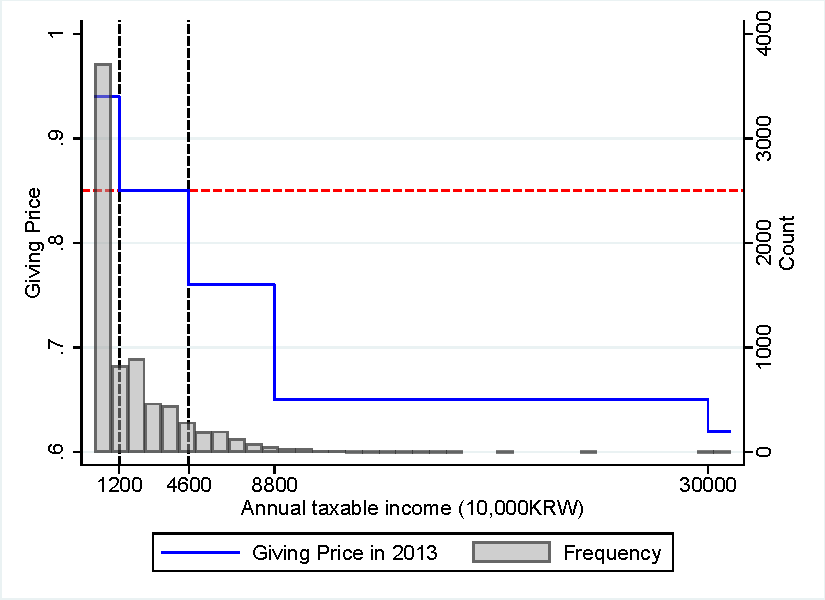
\includegraphics[width=0.9\linewidth]{C:/Users/katoo/Desktop/NASTAB/_assets/SummaryPriceChange} 

  }

  \caption{Income Distribution and Giving Price in 2013}\label{fig:unnamed-chunk-2}
  \end{figure}

  \clearpage

  \hypertarget{references}{%
  \subsection*{References}\label{references}}
  \addcontentsline{toc}{subsection}{References}

  \hypertarget{refs}{}
  \begin{CSLReferences}{1}{0}
  \leavevmode\hypertarget{ref-Bursztyn2017}{}%
  Bursztyn, L., Jensen, R., 2017. Social image and economic behavior in the field: Identifying, understanding, and shaping social pressure. Annual Review of Economics 9, 131--153. doi:\href{https://doi.org/10.1146/annurev-economics-063016-103625}{10.1146/annurev-economics-063016-103625}

  \end{CSLReferences}

\end{document}

